\chapter{Vibração induzida por vórtices em vãos livres}

Quando um fluido de baixa viscosidade encontra um obstáculo, forma-se uma camada limite.
Esta fina camada de fluido está sujeita aos efeitos das forças viscosas.
Nesta camada a velocidade do fluxo varia rapidamente, ficando cada vez mais lenta, formando um escoamento rotacional dentro da camada limite.
Para determinadas velocidades de escoamento, a camada limite se desprende do obstáculo, formando uma esteira de vórtices, conhecida como esteira de von Kármán~\cite{Currie2002}, conforme visto na Figura~\ref{fig:viv_shading}.
Como consequência direta do desprendimento de vórtices, surge uma força oscilatória transversal ao fluxo, que age sobre o obstáculo, resultando em oscilações verticais e horizontais~\cite{Nielsen2002}.

\begin{figure}[!ht]
    \centering
    \caption{Esteira de Von Kármán.}\label{fig:viv_shading}
    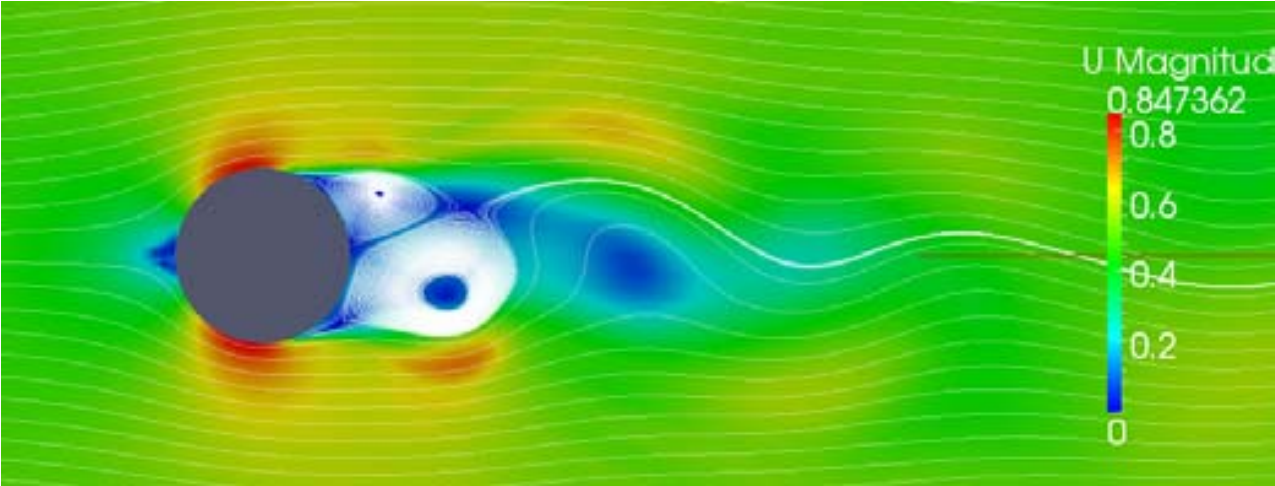
\includegraphics[width=0.6\textwidth]{imagens/viv_shading}
    \\Fonte:~\citeonline{VandenAbeele2013}.
\end{figure}

A frequência do desprendimento de vórtices causado por um fluxo normal ao obstáculo (o duto em vão livre, no caso em questão), é governado pelo número de Strouhal, diâmetro externo e velocidade de fluxo~\cite{Mork2003}.
O número de Strouhal pode ser obtido pela expressão $S_t = (f L) / V$, onde $f$ é a frequência de vórtices, $L$ é o comprimento característico e $V$ é a velocidade do fluxo.
Quando a velocidade do fluxo alcança uma das frequências naturais da estrutura, ela começa a vibrar e estas duas vibrações se correlacionam, causando vibrações de grande amplitude e grande dano (\textit{lock-in})~\cite{Mork2003}.

Como os dutos são geralmente modelados como cilindros, é importante entender como funciona o comportamento do fluxo de fluido ao redor dessa estrutura. Segundo \apudonline{Sumer1995}{Batchelor1967}, ao estudar vibrações de cilindros em corrente constante, inicia-se o desprendimento de vórtices quando o número de Reynolds, $R_e = (U\cdot D)/\nu$, é maior que $40$, onde $U$ é a velocidade do fluxo, $D$ é o diâmetro do cilindro e $\nu$ é a viscosidade cinemática~\cite{Sumer1995}.

O desprendimento de vórtices induz uma variação cíclica de forças no cilindro.
Assim, enquanto uma força de sustentação (\textit{lift force}) oscila à mesma frequência do desprendimento de vórtices, a força de arrasto (\textit{drag force}) oscila à duas vezes esta mesma frequência~\cite{Sumer1995}.
Estas forças oscilatórias, os vórtices, podem induzir vibrações na direção ortogonal ao fluxo, \textit{cross-flow} (CF), e na direção do fluxo, \textit{in-line} (IL), denominadas: vibrações induzidas por vórtices (VIV).

Os diversos dutos submarinos, que tem como objetivo o transporte de fluidos, seja entre o poço e a plataforma, entre plataformas etc., estão sujeitos ao fluxo intermitente de cargas ambientais.
Essas cargas, tornam-se um desafio ainda maior quando os dutos, instalados diretamente no irregular leito marinho, encontram-se em vãos livres~\cite{Fyrileiv1998}, como ilustrado na~\autoref{fig:freespan}.

\begin{figure}[!ht]
	\centering
    \caption{Duto em Vão livre e direções das oscilações.}\label{fig:freespan}
	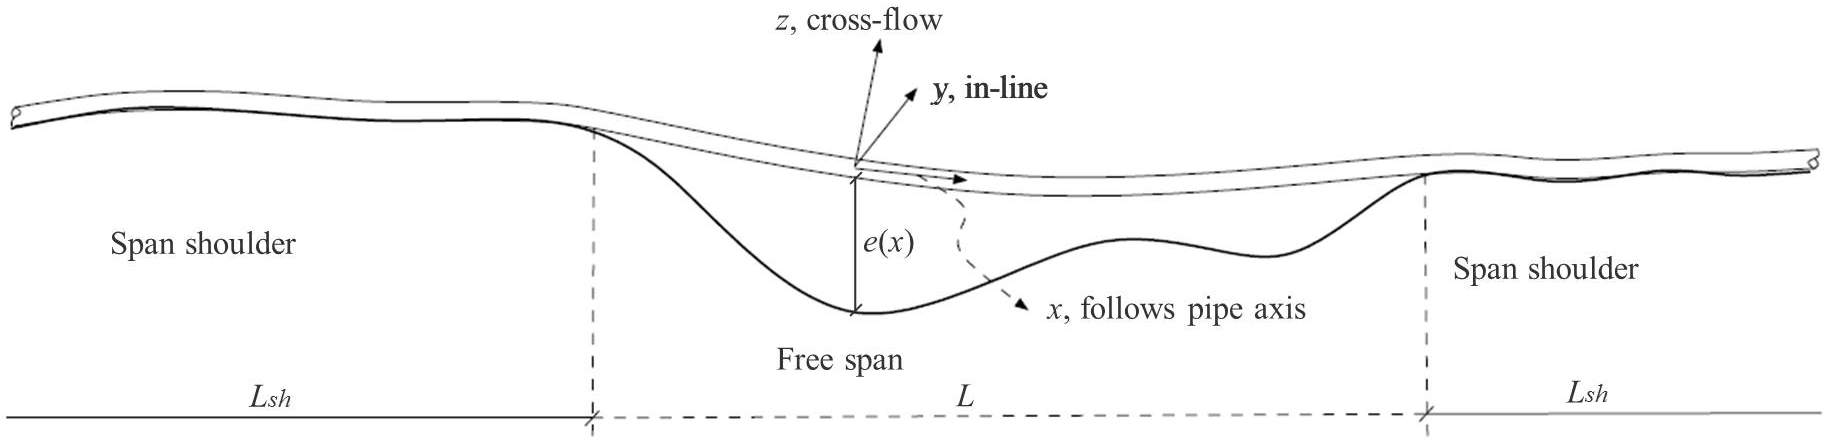
\includegraphics[width=1\textwidth]{imagens/freespan}
    \\Fonte:~\citeonline{DNV2017}.
\end{figure}

Porém, vãos livres não aparecem apenas quando os dutos são instalados em leito irregular, mas também quando ocorre erosão posterior (\textit{scouring}\footnote{Erosão do solo marinho causada pela ação de ondas ou correntes. Caracteriza-se pela remoção de sedimentos com formação de cavidades ou canais.}), devido, por exemplo, a suportes artificiais.
Com o duto exposto à ondas e correntes, a parte não apoiada estará suscetível à VIV.\@
Caso a frequência de desprendimento alcance uma das frequências naturais do duto, esse poderá entrar em ressonância.
As excitações dinâmicas podem causar danos por fadiga, sendo importante identificar os corretos procedimentos de intervenção, seja no duto ou no leito marinho.

A \dnvf105 utiliza uma metodologia baseada em modelos de resposta a fim de avaliar a fadiga causada por VIV em dutos em vão livre.
Estes modelos representam relações empíricas entre a velocidade reduzida (\autoref{eq:viv-Vr}) e a amplitude de resposta adimensional, utilizadas para prever as amplitudes de vibração nas direções \textit{in-line} e \textit{cross-flow}~\cite{Mork2003,DNV2017}.
Além desta, a recomendação prática sugere também um método baseado no coeficiente de sustentação e nas curvas do coeficiente de massa adicional como função da amplitude de resposta adimensional e da frequência de vibração adimensional~\cite{DNV2017}.
Como terceira opção, a \dnvf105 indica o uso de fluidodinâmica computacional (CFD, na sigla em inglês) para escoamento turbulento ao redor dos dutos para avaliação do VIV.\@

A \dnvf105 considera dois modelos para estimar a resposta dinâmica em um vão livre: Modelo de Resposta (\textit{Response Model} - RM) e Modelo de Força (\textit{Force Model} - FM).
A escolha do modelo, segundo~\citeonline{Tura1994}, depende: (i) do comportamento dos carregamentos ambientais, isto é, quando há ressonância induzida por vórtice, aplica-se RM; e quando o comportamento do vão livre é afetado por carregamentos periódicos com pouca ou nenhuma amplificação dinâmica, aplica-se FM; (ii) da direção e tipo de fluxo, RM é aplicável na direção \textit{in-line} para corrente contínua e na direção \textit{cross-flow} para qualquer padrão de fluxo; o FM é aplicado na direção \textit{in-line} para carregamentos de onda direto.

% Caracteriza-se \textit{single mode} quando há um único valor para amplitude de corrente, sem que haja variações com a direção, e não houver presença de ondas.
A \dnvf105 pode ser aplicada para vãos únicos e múltiplos onde um modo de vibração é predominante (\textit{single-mode}), conforme a \autoref{fig:vaos_tipicos}.
Porém, a combinação de vãos de grande extensão e altas correntes, ou ainda vãos múltiplos, faz com que não apenas os modos fundamentais sejam ativados, mas também diversos outros modos de ordem mais alta (\textit{multi-mode}).

\begin{figure}[!ht]
	\centering
    \caption{Configurações típicas para vãos.}\label{fig:vaos_tipicos}
	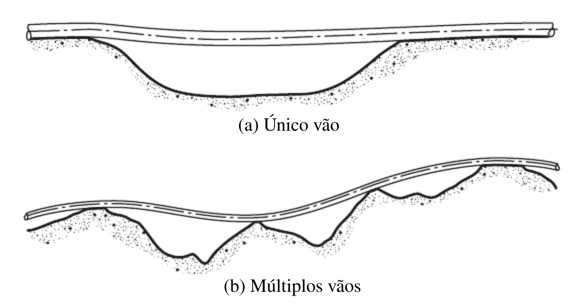
\includegraphics[width=0.7\textwidth]{imagens/vaos_tipicos}
    \\Fonte:~\citeonline{Bai2014}.
\end{figure}

A primeira etapa do cálculo das frequências de vibração dos dutos em vão livre é o cálculo da força axial efetiva, $S_\mathit{eff}$, e os parâmetros de rigidez do solo $K_v$, $K_l$ calculados por meio das Equações~\ref{eq:viv-Kv} e~\ref{eq:viv-Kl}, sendo $K_\mathrm{v,s}$ um valor tabelado de acordo com o tipo de solo escolhido.

Com o intuito de demonstrar a formulação do modelo de resposta para o caso \textit{single mode} de um duto totalmente restringido, tem-se que a tensão axial efetiva é dada por
\begin{equation}
\label{eq:viv-Seff}
S_\mathit{eff} = H_\mathit{eff} - \Delta p_i A_i (1 - 2\nu) - A_s E \Delta T \alpha_E
\end{equation}
onde

\begin{tabular}{rl}
$H_\mathit{eff}$ & tensão efetiva de lançamento\\
$\Delta p_i$     & diferencial de pressão interna em relação ao lançamento\\
$A_i$            & área da seção transversal interna do duto de aço\\
$\nu$            & coeficiente de Poisson\\
$A_s$            & área da seção transversal externa do duto de aço\\
$E$              & módulo de elasticidade\\
$\Delta T$       & diferencial de temperatura em relação ao lançamento\\
$\alpha_E$       & coeficiente de expansão de temperatura
\end{tabular}

Em seguida, calcula-se a carga crítica de flambagem, definida como
\begin{equation}
\label{eq:viv-Pcr}
P_\mathit{cr} = (1 + \mathit{CSF}) C_2\pi^2 \mathit{EI}/L_\mathit{eff}^2
\end{equation}
com
\begin{equation}
\label{eq:viv-CSF}
\mathit{CSF} = k_c {\left(\frac{\mathit{EI}_\mathit{conc}}{\mathit{EI}}\right)}^{0,75}
\end{equation}
onde

\begin{tabular}{rl}
	$\mathit{CSF}$               & fator de rigidez do concreto\\
	$C_2$                        & coeficiente das condições de contorno\\
	$\mathit{EI}$                & rigidez à flexão do aço\\
	$L_\mathit{eff}$             & comprimento efetivo do vão\\
	$k_c$                        & constante empírica para a rigidez do concreto\\
	$\mathit{EI}_\mathit{conc}$  & rigidez à flexão do concreto
\end{tabular}

A constante empírica $k_c$ considera a deformação/deslizamento no revestimento anti-corrosão e as fraturas no revestimento de concreto.

O comprimento efetivo do vão, dado pelo produto do comprimento do vão por um fator de escala, é necessário visto que as condições de contorno nos ombros (\textit{shoulders}) que o duto se apoia estão entre \textit{pinned-pinned} e \textit{fixed-fixed}\footnote{Valores dos fatores $C_1$ a $C_6$ estão dispostos na Tabela 6-1~cite[p. 111]{DNV2017}, e só devem ser utilizados apenas para cenários \textit{single-span}.}.
Logo, temos que
\begin{equation}
\label{eq:viv-LeffL}
\frac{L_\mathrm{eff}}{L} =
\begin{cases}
	4,73 / (-0,066 \beta^2 + 1,02 \beta + 0,63)   & \mathrm{para} \beta \geq 2,7 \\
	4,73 / (0,036 \beta^2 + 0,61 \beta + 1)       & \mathrm{para} \beta <    2,7
\end{cases}
\end{equation}
com
\begin{equation}
\label{eq:viv-beta}
\beta = \log_{10}\left( \frac{K L^4}{(1 + \mathit{CSF})\mathit{EI}_\mathit{conc}} \right)
\end{equation}
onde $L$ é o comprimento real do vão e $K$ é a rigidez estática ou dinâmica do solo por unidade de comprimento.

Pode-se encontrar o módulo de Young do concreto a partir da expressão
\begin{equation}
\label{eq:viv-Econc}
E_\mathit{conc} = 10000 f_\mathit{cn}^{0,3}
\end{equation}
onde $f_\mathit{cn}$ é a resistência de fabricação do concreto.

Os parâmetros de rigidez do solo são calculado com base na DNVGL-RP-F114~\cite{DNVF114}.
A rigidez dinâmica do solo por metro na direção vertical (\textit{cross-flow}) é dada por
\begin{equation}
\label{eq:viv-Kv}
K_v = \frac{C_v}{1 - \nu_\mathit{soil}}\left(\frac{2}{3}\frac{\rho_s}{\rho}+\frac{1}{3}\right)\sqrt[]{D}
\end{equation}
e a rigidez dinâmica do solo por metro na direção lateral (\textit{in-line}) por
\begin{equation}
\label{eq:viv-Kl}
K_l = C_l (1+\nu_\mathit{soil})\left(\frac{2}{3}\frac{\rho_s}{\rho}+ \frac{1}{3}\right)\sqrt[]{D}
\end{equation}
onde

\begin{tabular}{rl}
	$C_v$               & fator de rigidez dinâmica do solo na direção vertical\\
	$C_l$               & fator de rigidez dinâmica do solo na direção longitudinal\\
	$\nu_\mathit{soil}$ & coeficiente de Poisson do solo\\
	$\rho_s$            & massa específica do duto\\
	$\rho$              & massa específica da água deslocada\\
	$D$                 & diâmetro externo do duto (incluindo revestimento)
\end{tabular}

Caso não seja um dado advindo das medições, ou estimado analiticamente, é necessário calcular a deflexão estática \textit{mid-span}, que é dada por
\begin{equation}
\label{eq:viv-deflex}
\delta = C_6 \frac{q L_\mathit{eff}^4}{\mathit{EI} (1 + \mathit{CSF})} \frac{1}{S_\mathit{eff}/P_\mathit{cr}}
\end{equation}
onde $C_6$ é um coeficiente da condição de contorno e $q$ é o peso submerso.

A frequência natural fundamental, a ser definida para as direções \textit{in-line} e \textit{cross-flow}, pode ser aproximada a partir de
\begin{equation}
\label{eq:viv-f1}
f_1 \approx C_1 \sqrt{1 + \mathit{CSF}}\sqrt{\frac{\mathit{EI}}{m_e} L_\mathit{eff}^4} \left(1 + \frac{S_\mathit{eff}}{P_\mathit{cr}} + C_3 {\left(\frac{\delta}{D}\right)}^2\right)
\end{equation}
onde $C_1$ e $C_3$ são coeficientes de condições de contorno e $m_e$ é a massa efetiva, incluindo a massa estrutural, massa do fluido interno e massa adicional.

Desta forma, o efeito da massa adicional pode ser modelado a partir do coeficiente de massa adicional ($C_a$), que pode ser aplicado para superfícies suaves ou rugosas do duto e deve ser aplicada para frequência natural da água parada, sendo calculado da seguinte forma
\begin{equation}
\label{eq:viv-Ca}
C_a =
\begin{cases}
	0,68 + \frac{1,6}{1 + 5 (e/D)} & \mathrm{para} e/D < 0,8 \\
	1                              & \mathrm{para} e/D \geq 0,8
\end{cases}
\end{equation}
onde $e$ corresponde ao \textit{gap} do vão, isto é, a distância entre o duto e o solo marinho.

Além disto, podem-se calcular também a amplitude máxima de tensão para o diâmetro unitário para os modos fundamentais \textit{in-line} ($\mathit{IL}$) e \textit{cross-flow} ($\mathit{CF}$) assim
\begin{equation}
\label{eq:viv-Ailcf}
A_{\mathit{IL}/\mathit{CF}, 1}^{\max} = 2 C_4(1 + \mathit{CSF})\frac{D E r}{L_\mathit{eff}^2}
\end{equation}
em que $r$ é uma coordenada radial da seção transversal do duto e $C_4$ é um coeficiente de condição de contorno.


Por fim, finaliza-se esta etapa com o cálculo do fator de redução para corrente, $R_C$, que será aplicado na velocidade de referência, sendo calculado assim
\begin{equation}
\label{eq:viv-R_C}
R_C(z) = R_c \frac{\ln(z)-\ln(z_0)}{\ln(z_r)-\ln(z_0)}
\end{equation}
com o fator de referência dado por
\begin{equation}
\nonumber
R_c = \sin(\theta_\mathit{rel})
\end{equation}
onde $z$ é a altura acima do solo, $z_0$ é o parâmetro de rugosidade, $z_r$ é a altura de medição de referência e $\theta_\mathit{rel}$ é o ângulo formado entre a corrente e o duto.

Podemos utilizar os resultados das equações acima para a construção dos modelos de resposta relacionando a velocidade do fluxo com a amplitude de vibração.
Pela \dnvf105, as vibrações \textit{in-line} e \textit{cross-flow} devem ser consideradas em modelos de resposta separados.


\section{Modelo de resposta \textit{in-line}}\label{sec:modelo-resposta-inline}

O parâmetro de estabilidade, $K_S$, representa o amortecimento para uma dada forma modal, sendo obtido a partir da equação
\begin{equation}
\label{eq:viv-Ks}
K_S = \frac{4 \pi m_e \zeta_T}{\rho_w D^2}
\end{equation}
em que $\rho_w$ é a densidade da água e $\zeta_T$ é a taxa de amortecimento modal total.
Aplica-se um fator de segurança ao parâmetro de estabilidade, $K_\mathit{Sd} = K_S/\gamma_k$, sendo $\gamma_k$ o fator de segurança no parâmetro de estabilidade.

Em seguida, deve-se calcular os fatores de correção para considerar a turbulência e o ângulo de ataque do fluxo
\begin{equation}
\label{eq:viv-Riot}
\begin{aligned}
    R_{I\theta,1} &= 1 - \pi^2\left(\frac{\pi}{2} - \sqrt{2 \theta_\mathit{rel}}\right)(I_c - 0,03) & \quad \mbox 0 \leq R_{I\theta,1} \leq 1\\
    R_{I\theta,2} &= 1 - \frac{I_c - 0,03}{0,17}                                                    & \quad \mbox  0 \leq R_{I\theta,2} \leq 1
\end{aligned}
\end{equation}
onde $I_c$ é a intensidade de turbulência.

Segundo a \dnvf105 o fluxo pode ser dividido em duas zonas: (i) uma zona exterior, distante do solo marinho, onde velocidade de corrente média e a turbulência variam muito pouco na direção horizontal, e (ii) uma zona interior, onde a velocidade de corrente média e a turbulência têm variações consideráveis na direção horizontal. Uma vez que as medições da corrente são realizadas na zona exterior, fora da camada limite, a velocidade de corrente no duto pode ser aproximada a partir da equação
\begin{equation}
\label{eq:vel-corrente}
U_c = R_c U(z_r) \frac{\ln{(e+D/2)} - \ln(z_0)}{\ln (z_r)- \ln (z_0)}
\end{equation}
em que $U(z_r)$ é a velocidade da corrente na altura de referência.

Uma vez encontrada a velocidade da corrente na zona interior, isto é, próxima do solo, a velocidade reduzida pode ser calculada assim
\begin{equation}
\label{eq:viv-Vr}
V_R = \frac{U_c + U_w}{f_n D}
\end{equation}
onde $U_w$ é a velocidade de fluxo induzida por onda e $f_n$ é a frequência natural de amplitude.

A amplitude de resposta \textit{in-line} depende da  (\autoref{eq:viv-Vr}), $V_R$, do parâmetro de estabilidade, $K_\mathit{Sd}$, da intensidade da turbulência, $\mathit{I}_c$, e do ângulo do fluxo, $\theta_\mathit{rel}$.
O modelo de resposta pode então ser construído através do conjunto de equações a seguir

\begin{equation}
\label{eq:viv-Vronset}
\frac{A_{Y,1}}{D} = \max\left(0,18 \left(1 - \frac{K_\mathit{Sd}}{1,2}\right) R_{I\theta,1} ~,~\frac{A_{Y,2}}{D}\right)\\
\end{equation}

\begin{equation}
\frac{A_{Y,2}}{D} = 0,13 \left(1 - \frac{K_\mathit{Sd}}{1,8}\right) R_{I\theta,2}\\
\end{equation}

\begin{equation}
V_{R,\mathit{onset}}^\mathit{IL} =
\begin{cases}
\frac{1}{ \gamma_{\mathit{on}, \mathit{IL}} }                 & \mathrm{para} K_\mathit{Sd} < 0,4\\
\\
\frac{0,6 + K_\mathit{Sd}}{\gamma_{\mathit{on}, \mathit{IL}}} & \mathrm{para} 0,4 \leq K_\mathit{Sd} < 1,6 \\
\\
\frac{2,2}{\gamma_{\mathit{on}, \mathit{IL}}}                 & \mathrm{para} K_\mathit{Sd} \geq 1,6
\end{cases}
\end{equation}

\begin{equation}
V_{R, \mathit{end}}^\mathit{IL} =
\begin{cases}
4,5 - 0,8 K_\mathit{Sd} & \mathrm{para} K_\mathit{Sd} < 1,0 \\
3,7                     & \mathrm{para} K_\mathit{Sd} \geq 1,0
\end{cases}
\end{equation}

\begin{equation}
V_{R, 1}^\mathit{IL} = 10 \left(\frac{A_{Y, 1}}{D}\right)+ V_{R,\mathit{onset}}^\mathit{IL}\\
\end{equation}

\begin{equation}
V_{R, 2}^\mathit{IL} =  V_{R, \mathit{end}}^\mathit{IL} - 2 \left(\frac{A_{Y, 2}}{D}\right)\\
\end{equation}

onde $\gamma_{\mathit{on}, \mathit{IL}}$ é o fator de segurança para velocidade de corrente inicial \textit{in-line} e $\frac{A_Y}{D}$ é a amplitude \textit{in-line} normalizada. Com esses valores calculados, pode-se construir a curva que relaciona velocidade reduzida e amplitude de vibração para diâmetro unitário, semelhante a \autoref{fig:viv-responsemodelil}.

\begin{figure}[!ht]
    \centering
    \caption{Curva de modelo de resposta \textit{in-line}.}\label{fig:viv-responsemodelil}
    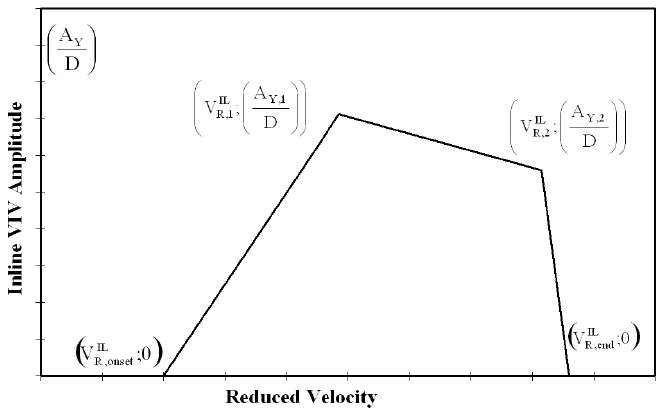
\includegraphics[width=0.8\linewidth]{imagens/response_model_IL}
    \\Fonte:~\citeonline{DNV2017}.
\end{figure}

Conforme observado na \dnvf105, a resposta de amplitude de um duto vibrando na direção \textit{in-line}, contempla regiões com velocidade de corrente entre 1,0 e 4,5.
Temos então que a resposta na direção longitudinal depende dos parâmetros de velocidade de corrente, estabilidade, intensidade de turbulência e do ângulo entre a corrente e o duto.
Percebe-se que, à medida em que o parâmetro de estabilidade aumenta, a amplitude de resposta tende à diminuir, uma vez que este é proporcional ao amortecimento do sistema~(\autoref{eq:viv-Ks}).


\section{Modelo de resposta \textit{cross-flow}}

Para o modelo de resposta \textit{cross-flow} também  é necessário calcular um conjunto de parâmetros. Dessa vez, inicia-se com o cálculo do fator de correção para considerar a proximidade do duto com o solo
\begin{equation}
\label{eq:viv-Psi}
\Psi_{\mathit{proxi}, \mathit{onset}} =
\begin{cases}
\frac{1}{5}\left(4 + 1,25\frac{e}{D} \right) & \mathrm{para}~\frac{e}{D} < 0,8\\
1                                            & \mathrm{caso~contr\acute{a}rio}
\end{cases}
\end{equation}

Caso o duto esteja localizado próximo ou em trincheiras é necessário considerar o fator de correção específico

\begin{equation}
\label{eq:viv-Psitren}
\Psi_{\mathit{trench}, \mathit{onset}} = 1 + 0,5\frac{\Delta}{D}
\end{equation}
onde $\Delta$ é a profundidade da trincheira.

O número de Keulegan-Carpenter é definido como
\begin{equation}
\label{eq:viv-KC}
\mathit{KC} = \frac{U_w}{f_w D}
\end{equation}
onde $f_w = \frac{1}{T_u}$ é o período de cruzamento da frequência de onda.

A razão de velocidade de fluxo de corrente é dada por
\begin{equation}
\label{eq:viv-alfa}
\alpha = \frac{U_c}{U_c + U_w}
\end{equation}

A partir dessas equações, se pode construir o modelo de resposta \textit{cross-flow} através do conjunto de equações a abaixo
\begin{equation}
\label{eq:viv-azdj}
\frac{A_{Z,1}}{D} =
\left\{
\begin{array}{ccc}
0,9                                                      & \alpha > 0,8   &         \frac{f_{n+1,CF}}{f_{n,CF}} <   1,5 \\
0,9 + 0,5 \left(\frac{f_{n+1,CF}}{f_{n,CF}} - 1,5\right) & \alpha > 0,8   & 1,5 \le \frac{f_{n+1,CF}}{f_{n,CF}} \le 2,3 \\
1,3                                                      & \alpha > 0,8   &         \frac{f_{n+1,CF}}{f_{n,CF}} >   2,3 \\
0,9                                                      & \alpha \le 0,8 &        \mathit{KC} >   30 \\
0,7 + 0,01 (\mathit{KC} -10)                             & \alpha \le 0,8 & 10 \le \mathit{KC} \le 30 \\
0,7                                                      & \alpha \le 0,8 &        \mathit{KC} <   10
\end{array}
\right.
\end{equation}

\begin{equation}
\frac{A_{Z,2}}{D} = \frac{A_{Z,1}}{D}
\end{equation}

\begin{equation}
V_{R,\mathit{onset}}^\mathit{CF} = \frac{3 \cdot \Psi_{\mathit{proxi}, \mathit{onset}} \cdot  \Psi_{\mathit{trench}, \mathit{onset}}}{\gamma_{\mathit{on}, \mathit{CF}}}
\end{equation}

\begin{equation}
V_{R,\mathit{end}}^\mathit{CF} = 16
\end{equation}

\begin{equation}
V_{R, 1}^\mathit{CF} = 7 - \frac{7 - V^\mathit{CF}_{R, \mathit{onset}}}{1,15} \left(1,3 - \frac{A_{Z,1}}{D}\right)
\end{equation}

\begin{equation}
V_{R, 2}^\mathit{CF} = V^\mathit{CF}_{R, \mathit{end}} - \frac{7}{1,3} \frac{A_{Z, 1}}{D}\\
\end{equation}

Com esses valores calculados, pode-se construir a curva que relaciona velocidade reduzida e amplitude de vibração para diâmetro unitário, semelhante a \autoref{fig:viv-responsemodelcf}.

\begin{figure}[!ht]
    \centering
    \caption{Curva de modelo de resposta \textit{cross-flow}.}\label{fig:viv-responsemodelcf}
    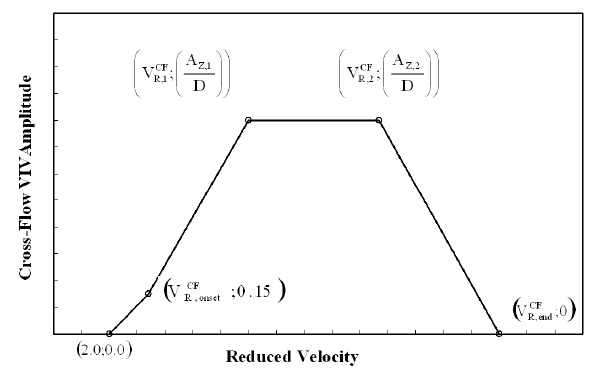
\includegraphics[width=0.8\linewidth]{imagens/response_model_CF}
    \\Fonte:~\citeonline{DNV2017}.
\end{figure}


\section{\label{sec:multimode}Resposta \textit{multi-mode}}

A resposta do vão livre pode ser dada em função de uma coordenada $x$ ao longo da direção longitudinal do duto.
Para cada combinação relevante de estado de mar e velocidade de corrente, um número de modos pode ser excitado simultaneamente na mesma direção, dando origem a uma resposta \textit{multi-mode}.
Todavia, o número de modos que responderão e o quanto cada modo contribuirá para o dano por fadiga dependerá da velocidade do fluxo, da posição no eixo $x$ e da competição com outros modos.

A \dnvf105 define três diferentes tipos de modos:
\begin{description}
	\item[Modos ativos] são os modos que podem ser excitados por VIV. Com base no itém 2.3.3 da DNVGL-RP-F105, os critério para definição de para que um modo \textit{in-line}, com frequência $f_{IL,j}$, ou \textit{cross-flow}, com frequência $f_{CF,j}$, seja considerado ativo é:

    \begin{equation}
        \begin{aligned}
        f_{I L, j} & \leq \frac{U_{\text{extreme}} \gamma_{f,IL}}{V_{R,\text{onset}}^{IL} D} \\
        f_{C F, j} & \leq \frac{U_{\text{extreme}} \gamma_{f,CF}}{2D}
        \end{aligned}
    \end{equation}
    sendo $\gamma_{f,IL}$ e $\gamma_{f,CF}$ coeficientes de segurança, variando de 1 a 1,3 a depender da classe de segurança e nível de
    definição do vão livre (item 2.7.2 da DNVGL-RP-F105).
    Um modo que não passível de ativação pode ser totalmente desconsiderado nas análises em todos os pontos e velocidades de fluxo.

    \item[Modos participantes] são modos ativos que têm amplitude de tensão relevante em um, ou ambos os lados, de um ponto x. Para que um modo j seja considerado participante no vão, é necessário que a seguinte condição (presente no item 4.3.3) seja atendida:
    $$
    \left|A_{\textbf{IL/CF}, j}(x)\right| \geq \frac{A_{IL/CF}^{\max}}{10} \text{ para algum } x \in (x_{\text{start},j}, x_{\text{end}, j})
    $$
    sendo
    $$
    A_{IL/CF, j}(x) = (1+CSF) D \kappa_{j}(x) E r
    $$
    onde

    \begin{tabular}{rl}
        $\mathit{CSF}$                            & fator de rigidez do concreto\\
        $\kappa_{j}(x)$                           & curvatura do modo na posição $x$\\
        $E$                                       & módulo de elasticidade\\
        $r$                                       & coordenada radial da seção transversal do duto\\
        $(x_{\text{start},j}, x_{\text{end}, j})$ & intervalo de influência do modo
    \end{tabular}

	\item [Modos contribuintes] são modos participantes que deve satisfizer um dos seguintes critérios:

        \begin{itemize}
    	\item direção \textit{cross-flow}: ${(A_Z/D)}_j \geq 0,1{(A_Z/D)}_{\max}$

        \item direção \textit{in-line}: $S_{\mathit{IL}, \mathit{j}}^{P}(x) \geq 0,1 S_\mathit{IL}^{\max}(x)$
        \end{itemize}

	onde ${(A_Z/D)}_j$ é a amplitude VIV normalizada para o j-ésimo modo, ${(A_Z/D)}_{\max}$ é a amplitude VIV normalizada para o modo \textit{cross-flow}  dominante, $S_{\mathit{IL}, \mathit{j}}^{P}(x)$ é a amplitude de tensões de reposta preliminar para o j-ésimo modo \textit{in-line} e $S_\mathit{IL}^{\max}(x)$ é a amplitude de tensões de resposta associadas ao modo \textit{in-line} dominante.

\end{description}

Baseado nos modelos de resposta \textit{single-mode}, podemos calcular as amplitudes do VIV para todos os modos (\autoref{procedure_il}).
Assim, precisamos calcular VIV \textit{cross-flow} e \textit{in-line} para cada velocidade de corrente, estado de mar e em cada ponto com se os seguintes procedimentos:

\begin{itemize}

\item VIV \textit{cross-flow}\label{procedure_il}

\begin{enumerate}
\item Identifica-se todos os modos participantes (\textit{single} ou \textit{multi location})

\item Com o modelo de resposta \textit{cross-flow}:
	\begin{enumerate}
    \item Calcula-se a amplitude VIV normalizada para cada modo ${(A_Z/D)}_j$

	\item Identifica-se o modo dominante, isto é, ${(A_Z/D)}_{\max}$

    \item Identificam-se os modos fracos $0,1{(A_Z/D)}_{\max} \leq {(A_Z/D)}_j \leq {(A_Z/D)}_{\max}$

    \item Desconsidera-se os modos irrelevantes: ${(A_Z/D)}_j$ < $0,1{(A_Z/D)}_{\max}$
    \end{enumerate}

\item Usando o modelo de resposta para baixos valores de Keulegan-Carpenter (\textit{low Keulegan Carpenter flow regime} - LKCR), calcula-se ${(A_Z/D)}_j$ para cada modo.

\item Determina-se a resposta de tensão combinada:
    $$
    S_{\mathit{comb}, \mathit{CF}} = \max\left( S_{\mathit{comb}, \mathit{CF}}^\mathit{RM} ~,~ S_{\mathit{comb}, \mathit{CF}}^\mathit{LKCR} \right)
    $$

\item Determina-se a frequência de contagem de ciclos:

    $$
    f_{\mathit{cyc}, \mathit{CF}} =
    \begin{cases}
    f_{\mathit{cyc}, \mathit{CF}}^\mathit{LKCR}, & S_{\mathit{comb},\mathit{CF}}^\mathit{RM}(x)    < S_{\mathit{comb},\mathit{CF}}^\mathit{LKCR}(x) \\
    f_{\mathit{cyc}, \mathit{CF}}^\mathit{RM},   & S_{\mathit{comb},\mathit{CF}}^\mathit{RM}(x) \geq S_{\mathit{comb},\mathit{CF}}^\mathit{LKCR}(x)
    \end{cases}
    $$

\end{enumerate}

\item VIV \textit{in-line}

\begin{enumerate}
    \item Identifica-se todos os modos participantes (\textit{single} ou \textit{multi location})

    \item Com o modelo de resposta \textit{in-line}:

    \begin{enumerate}
    	\item Calcula-se a amplitude VIV normalizada para cada modo ${(A_Y/D)}_j$

    	\item Identifica-se o modo dominante, isto é, o modo com $S_\mathit{IL}^{\max}(x)$

    	\item Identificam-se potenciais modos fracos: $0,1 S_\mathit{IL}^{\max}(x) \leq S_{\mathit{IL}, \mathit{j}}^{P}(x) \leq S_\mathit{IL}^{\max}(x)$

    	\item Desconsideram-se os modos irrelevantes: $S_{\mathit{IL}, \mathit{j}}^{P}(x) < 0,1 S_\mathit{IL}^{\max}(x)$
    \end{enumerate}

        \item Reduzir os modos fracos.
        Para VIV \textit{in-line}, dois modos adjacentes podem competir se suas frequências forem próximas, ou agir de forma independente se estiverem distantes.
        A \dnvf105 define que os modos competem se a razão entre as frequências é menor que 2, isto é, $\frac{f_\mathit{n+1}}{f_n} < 2$.
        Em modos adjacentes considera-se que apenas o ``vencedor'' da competição pode ter máxima amplificação, enquanto a amplificação do modo ``perdedor'' é reduzida à metade. É interessante ressaltar que modos que não competem não têm redução.

        \item Calcular o intervalo de tensões \textit{in-line} excitados pelo modo \textit{cross-flow} dominante $S_{\mathit{\textit{cross-flow}}-\mathit{IL}}(x)$.

        Para cada ponto e cada modo, calcula-se o intervalo de tensões induzido por VIV \textit{in-line} para os modos contribuintes:
            \[S_{\mathit{IL}, \mathit{j}}^\mathit{RM}(x) = S_{\mathit{IL}, \mathit{j}}^{P} \cdot 0,5^{\beta_j (x)}\]

        Assume-se que apenas o modo \textit{cross-flow} dominante é capaz de contribuir para o movimento \textit{in-line} induzido pelo modo transversal.
        Desta forma, o modo \textit{in-line} participante cuja frequência natural é próxima a duas vezes a resposta \textit{cross-flow} dominante é escolhido como candidato a VIV \textit{in-line} induzido por \textit{cross-flow}.

        % \[\mid f_{\mathit{IL}, \mathit{k}}^\mathit{part} - 2 \cdot f_{\mathit{\textit{cross-flow}-RES}, \mathit{i}} \mid\]

        A amplitude de tensões \textit{in-line} excitados pelo modo \textit{cross-flow} dominante é dado por:

       	    \[S_{\mathit{CF-IL}}(x) = 0,8 \cdot A_{\mathit{IL}, \mathit{k}}~(x) \cdot {\left(\frac{A_{z}}{D}\right)}_{\max}~\cdot~R_k \cdot \gamma_s\]

    \item  Escolher o maior $S_\mathit{IL}^\mathit{RM}(x)$ e $S_{\mathit{CF-IL}}(x)$ para cada modo;

    \item Determinar a faixa de resposta de tensão combinada,

    \[S_{comb,IL}(x)=\sqrt{\sum_{j=1}^{m_{aig}}{\left(S_{IL,j}(x)\right)}^{2}}\]

    e a frequência de contagem de ciclos,

    \[f_{cyc,IL}(x)=\sqrt{\sum_{j=1}^{m_{\text{ug}}}{\left(f_{\text {IL}, j}^{con} \cdot \frac{S_{IL,j}(x)}{S_{comb,IL}(x)}\right)}^{2}}\]
    \end{enumerate}
\end{itemize}
